\chapter{Arquitecturas ILP}
Este capítulo trata sobre arquitecturas con paralelismo a nivel de instrucción (\emph{Instruction Level Parallelism}, ILP). Comentaremos una de las formas de incrementar el número de instrucciones por ciclo (IPC) en un procesador segmentado, que consiste en incrementar el número de instrucciones que se emiten a las unidades funcionales donde se ejecutan las operaciones que las instrucciones codifican.

Esta funcionalidad es perseguida tanto por procesadores superescalares como por procesadores VLIW, cuyas diferencias comenzaremos a destacar.

\section{Introducción}

\subsubsection{Nomenclatura}
Históricamente se utilizaba ``arquitectura de un computador'' para hacer referencia al repertorio de instrucciones que implementaba su procesador. Sin embargo, se comenzó a usar la palabra ``microarquitectura'' para ello, dejando la palabra ``arquitectura'' para denotar cómo está implementada la microarquitectura: qué unidades tiene, cómo están comunicadas entre sí, cómo funciona cada una, \ldots\\

A lo largo de esta sección hablaremos largo y tendido sobre cómo se ejecutan las instrucciones. Para ello, convenimos en decir que:
\begin{itemize}
    \item Una instrucción se está \underline{procesando} cuando está en alguna etapa del cauce de procesamiento de la misma.
    \item Una instrucción se está \underline{ejecutando} cuando está en la etapa de ejecución del cauce de procesamiento.
\end{itemize}
Finalmente, aconsejamos consultar la Sección~\ref{subsec:repaso_ILP}, antes de continuar con la lectura de este capítulo.

\subsection{Diferencias entre núcleos ILP}
En los núcleos que implementan paralelismo a nivel de instrucción (aquellos que son capaces de emitir más de una instrucción por ciclo), nos encontramos con dos grandes familias:
\begin{description}
    \item [Núcleos ILP superescalares.]~\\
        Replican alguna de las unidades funcionales del cauce de procesamiento de instrucciones. 

        De esta forma, es el hardware quien se encarga de la planificación de las instrucciones (decide qué instrucciones se emitirán a la vez en cada momento).
    \item [Núcleos ILP con VLIW.]~\\
        Donde VLIW significa \emph{Very Long Instruction Word}, estos procesadores realmente sólo emiten una instrucción por ciclo, pero cada una de ellas codifica varias operaciones (cada una correspondería a una instrucción en arquitecturas escalares). 

        Por tanto, no hay hardware que se encargue de la planificación de instrucciones, sino que es el software (los compiladores) quien se encarga de la planificación de instrucciones, generando instrucciones largas que contienen las operaciones que se emitirán juntas durante la ejecución.
\end{description}
Las dos implementaciones segmentan el procesamiento de las instrucciones en etapas, que se corresponden con las de la Sección~\ref{subsec:repaso_ILP}.\\

Debido al menor uso de hardware que requieren los núcleos VLIW, suelen usarse en computadores empotrados.\\

\section{Microarquitectura de ILP superescalares}
Las instrucciones se captan según el orden del programa, que pasan al buffer de instrucciones, donde esperan a decodificrase en este mismo orden. Una vez decodificada la instrucción, ya se saben los recursos a utilizar por la misma, por lo que pasa a la fase de emisión.

La emisión a ejecución puede realizarse con el orden del programa o de forma desordenada, con el fin de ahorrar tiempos de ejecución (suele hacerse lo segundo). Ya sea ordenada o no, como cada instrucción supone un tiempo distinto, la finalización de las instrucciones será desordenada. Esto es, podemos tener una instrucción que pase antes a ejecución y que termine después que una instrucción que entró después a ejecución, ya que esta segunda era mucho más corta que la primera.\\

En los superescalares, la última etapa del cauce de procesamiento de instrucciones (dedicada a \emph{write-back}) procesa las mismas de forma ordenada (según el orden del programa), a pesar de que se produzca una ejecución desordenada de las instrucciones.

Con esto, se garantiza la consistencia del procesador, de forma que el resultado tras ejecutar una serie de instrucciones coincida con el que provocaría la ejecución ordenada de las mismas.\\

La realidad es que cada una de las etapas desarrolladas en la Sección~\ref{subsec:repaso_ILP} se dividen a su vez en subetapas. Podemos encontrar implementaciones que realicen hasta 14 subetapas en las etapas más complejas.

\subsubsection{Dependencias y riesgos}
La segmentación nos permite disminuir el tiempo de ciclo de la CPU, reduciéndolo hasta en $N$ veces el tiempo de ciclo anterior, siendo $N$ el número de etapas del cauce (suponiendo que todas las etapas duran lo mismo).

Sin embargo, en los códigos a ejecutar nos encontramos con dependencias (de datos, de control o estructurales) que dan lugar a problemas en el cauce segmentado, los cuales pueden conducir a los programas a un resultado incorrecto en su ejecución. Todos estos problemas reciben el nombre de \emph{hazards} (o riesgos).\\

Para eliminar riesgos en los núcleos VLIW se deben introducir operaciones de no operación (\verb|nop|). Esto provoca una disminución en las prestaciones del núcleo (al desperdiciar ciclos de instrucción). Esta disminuición de las prestaciones es aún peor en los procesadores VLIW superescalares (núcleos capaces de dar por un ciclo varias instrucciones VLIW), donde obtenemos un IPC mucho mayor al introducir operaciones \verb|nop| que los que ya obteníamos en el VLIW escalar.

Todo esto sin considerar las dependencias estructurales (las cuales se detectan cuando en tiempo de ejecución dos instrucciones tratan de acceder a la misma unidad funcional), lo que ralentiza aún más los tiempos de ejecución.\\

A continuación, vamos a ver cómo en los computadores ILP superescalares es el hardware quien se encarga de eliminar los riesgos y de reducir el tiempo de penalización que suponen las dependencias, pudiendo llegar a un tiempo de ejecución próximo al ideal.

\subsection{Características del cauce de instrucciones}
Desarrollamos a continuación varios aspectos relevantes del cauce de procesamiento de instrucciones a tener en cuenta, los cuales \textbf{no han sido comentados en ninguna asignatura} hasta el momento. Podemos observar un cauce real en la Figura~\ref{fig:Cauce_ARM_cortex_a76}, donde la etapa de captación es la que se marca como \emph{Front End}, en color amarillo pastel; la etapa de decodificación y emisión la de color verde pastel; la de ejecución en verde oscuro y el \emph{write-back} en lila.

\begin{figure}
    \centering
    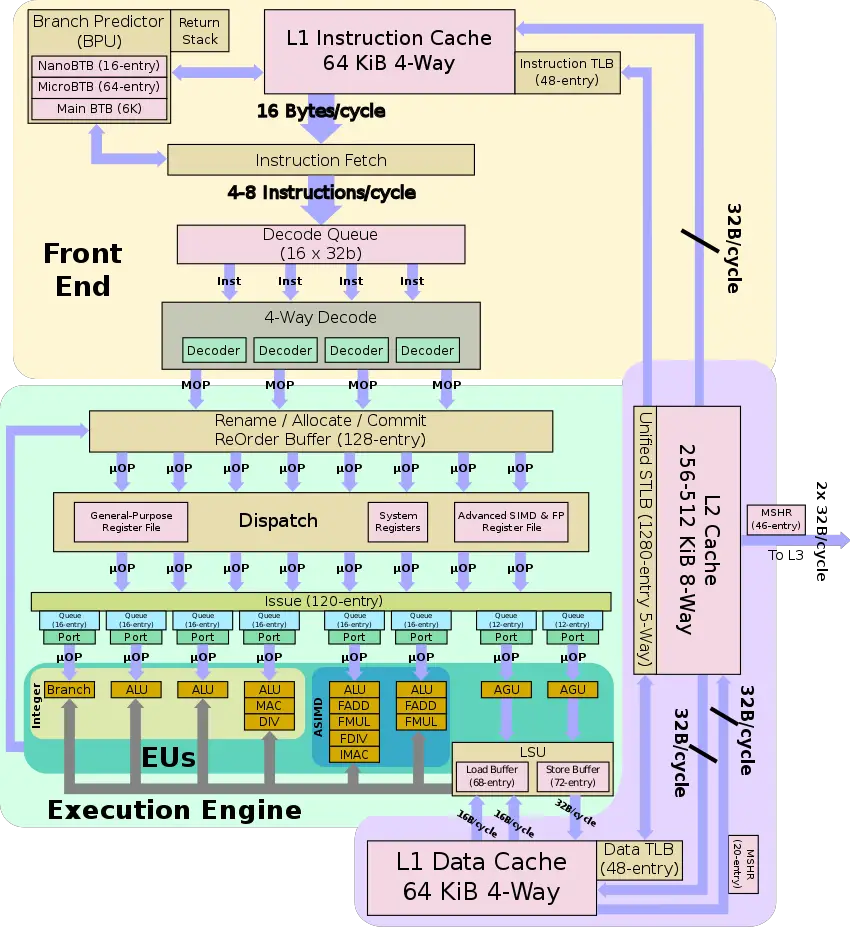
\includegraphics[width=0.8\linewidth]{Images/Cauce1.png}
    \caption{Cauce del procesador ARM cortex A76.}
    \label{fig:Cauce_ARM_cortex_a76}
\end{figure}

\begin{itemize}
    \item Como ya se comentaba en la Sección~\ref{subsec:repaso_ILP}, la etapa de ejecución y de memoria se consideraba una sola, al ser las instrucciones bien de acceso a memoria o bien instrucciones aritmético-lógicas.
    \item La etapa de emisión (aquella en la que ya se conocen los operandos y se prepara para mandar a ejecución) forma parte de la decodificación.
    \item Observamos que en la etapa amarillo pastel encontramos entre cada módulo y el siguiente 4 flechas representando puentes de datos, los cuales pasan a 8 en la etapa verde pastel. Esto sucede siempre en los x86 (son computadores CISC): sucede cuando una instrucción está implementada mediante varias microinstrucciones.
    \item En la etapa de emisión hay dos partes importantes: una en la que las instrucciones son almacenadas para su ejecución en lo que se llaman estaciones de reserva (o ventana de instrucciones en el caso de Intel), y una en la que se mandan a la primera unidad funcional desde las estaciones de reserva.
    \item En relación al punto anterior, Intel llama \textbf{emisión} a ventana de instrucciones y \textbf{envío} a unidades funcionales; mientras que manuales de ARM enuncian \textbf{envío} a estaciones de reserva y \textbf{emisión} a unidades funcionales.
    \item En la Figura~\ref{fig:Cauce_ARM_cortex_a76}, destacamos las unidades de \verb|AGU| y \verb|LSU|, que son las últimas a las que van a parar las instrucciones de acceso a memoria.
        \begin{itemize}
            \item Las \verb|AGU| son unidades de cálculo arimético que se encargan de calcular direcciones de acceso a memoria, la generación del address de una instrucción de acceso a memoria\footnote{Esta es la unidad que se encarga de procesar las instrucciones leaq de ASM, que se vieron en EC.}.
            \item Las \verb|LSU| son colas FIFO en las que esperan las instrucciones de acceso a memoria. Hay una cola dedicada a las instrucciones de lectura y otra a las de escritura. 
        \end{itemize}
    La implementación de adelantamiento de lecturas a escrituras propias (que vimos en el Capítulo~\ref{chapter:Tema3} que todos los procesadores incumplían en cuanto a orden global) se implementa en estas colas LSU\@. El protocolo genérico y más sencillo para realizarlo es el siguiente.

    Si viene una nueva instrucción y es de escritura, se introduce en su cola correspondiente. Si es de lectura, tenemos dos posibilidades:
    \begin{itemize}
        \item Si el cerebro de la \verb|LSU| no encuentra ninguna escritura con la misma dirección de memeoria en la cola de escrituras, simplemente se introduce en la cola correspondiente para lecturas.
        \item Si el cerebro de la \verb|LSU| detecta al menos una escritura a la última posición de memoria, coge el contenido de la última y se lo devuelve como resultado a la instrucción de lectura, sin llegar a leer dicha instrucción de memoria, al nunca introducirse en la cola.
    \end{itemize}
    Si los \verb|LSU| funcionan al igual que una cola FIFO (puede llevar quizás implementaciones más complejas, como sucede en los ARM), entonces los órdenes $W\rightarrow W$ y $R\rightarrow R$ son garantizados por el procesador (esto es lo que sucede en los Intel).

    Cabe destacar que la velocidad de las dos colas \verb|LSU| no es la misma, al avanzar las lecturas de forma más rápida que las escrituras.
\end{itemize}

\subsubsection{Unidades de cada etapa}

\begin{figure}
    \centering
    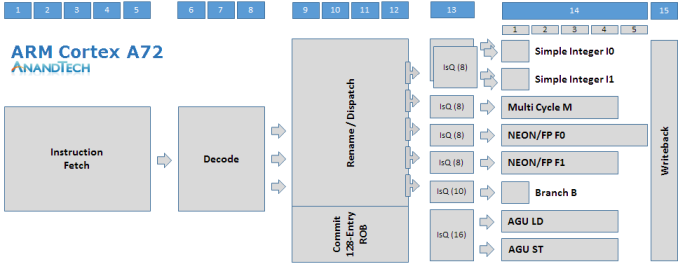
\includegraphics[width=0.8\linewidth]{Images/Cauce2.png}
    \caption{Cauce del procesador ARM cortex A72 de forma abstracta.}
    \label{fig:Cauce_ARM_cortex_a72}
\end{figure}

A continuación, en la Figura~\ref{fig:Cauce_ARM_cortex_a72} podemos volver a observar el cauce de instrucciones, esta vez de otro procesador similar, pero de una forma un tanto más abstracta. Procedemos a explicar qué unidades funcionales se encargan de realizar cada etapa, así como de explicar las funcionalidades y buffers de cada una, las cuales se desarrollarán en profundidad a lo largo del capítulo.

\begin{description}
    \item [Etapa de captación.] Formada por la unidad funcional etiquetada por ``Instruction Fetch'', recibe las instrucciones de la memoria caché L1 de instrucciones.

        Se encarga de detectar saltos y predecir saltos condicionales. Almacena la Tabla de saltos.
    \item [Etapa de decodificación y emisión.] Formada por las unidades funcionales de las columnas 6 a 12, recibe las instrucciones del IB (\emph{Instruction Buffer}), que sirve de puente entre la etapa de captación y esta.

        Se encarga primero de decodificar las instrucciones y luego de prepararlas para emisión (para enviarlas a las unidades funcionales), durante la cual (se desarrollarán pŕoximamente):
        \begin{itemize}
            \item Elimina riesgos WAW y WAR (renombrando registros con el buffer de renombrado).
            \item Elimina riesgos RAW y estructurales (mediante las estaciones de reserva).
            \item Reduce los riesgos de control (eejcución especulativa usando ROB).
            \item Captura de operandos desde registros de la arquitectura, o desde registros de renombrado.
        \end{itemize}
        Cuenta con la ventana de instrucciones o estación de reserva (las unidades de la columna 13, que preceden a la etapa de ejecución), con el Buffer de renombrado y con el Buffer de reorden (\emph{ReOrder Buffer} o ROB), que permite eliminar los riegos de control de forma sencilla. En el bloque de ``Rename/Dispatch'' tiene acceso a los registros de la arquitectura.
    \item [Etapa de ejecución.] Formada por todas las unidades de la columna 14, recibe las instrucciones de las ventanas de instrucciones o estaciones de reserva.
    \item [Etapa para \emph{write-barck}.] Formada por la unidad de la columna 15, implementa la consistencia secuencial del procesador así como la ejecución especulativa. Cuenta con un buffer de renombrado así como con el buffer de reorden (ROB).

        Además, elimina los riesgos de control que no fueron detectados por predicciones incorrectas (para ello usamos el ROB).
\end{description}

\subsection{Implementación de la etapa de emisión}
En esta sección, desarrollaremos en profundidad cómo funciona la etapa de emisión. Para ello, será necesario entender bien los buffers de renombrado, reorden y las estaciones de reserva, que son la parte principal de la etapa. Por simplicidad, en esta sección siempre que nos refiras a instrucciones, estaremos hablando de instrucciones aritméticas, que son las más completas para describir bien ambos buffers (por tener siempre un registro donde almacenar el resultado y operandos).

\subsubsection{Buffer de renombrado}
Cada vez que se emite una instrucción, se le asigna una entrada en la estación de reserva, y se renombra el registro en el que se va a guardar la salida de la instrucción (siempre se renombra), asignándole una entrada en el banco de registros de renombrado. Este banco se trata de una tabla de tantas entradas como registros, que contiene los siguientes campos (o columnas):

\begin{description}
    \item [Entrada válida.] Indica si la entrada de la tabla está en uso (se indica con un bit a 1) o no (bit a 0).
    \item [Registro de destino.] Se indica el registro que está siendo renombrado (un 3 en la entrada 5ª indica que el registro número 5 está renombrando al número 3).
    \item [Valor.] Se almacena el valor que se va a almacenar en el registro renombrado.
    \item [Valor válido.] Indica si el valor de la columna anterior es válido (esto es, que ha sido ya calculado), o no (la instrucción que da el valor fue emitida pero no terminó).
    \item [Último.] Si está activo indica que es el último renombrado de un registro. Por ejemplo, si el registro número 5 está siendo renombrado varias veces, la entrada que contenga un 1 en esta columna contendrá el valor válido para dicho registro.
\end{description}
A la hora de captar operandos, si necesitamos por ejemplo obtener el valor del registro 5, si este se encuentra renombrado (es decir, fue usado para almacenar el valor resultante de una operación), se captará el valor del buffer de renombrado (en caso de que tenga el bit de ``valor válido'' a 1, si no esperará). En caso contrario, se capta directamente del registro número 5.\\

Al renombrar siempre el registro que almacena el resultado de una instrucción, nunca podrán producirse dependencias de tipo WAW y WAR (eliminamos dichas depedencias), por lo que no es necesario detectarlas.

\begin{ejemplo}
    Supongamos que queremos ejecutar el siguiente código en el procesador:
    \begin{listing}[H]
    \begin{minted}[xleftmargin=6cm, linenos]{c++}
R3 = R3 - R5
R4 = R3 + 1
R3 = R5 + 1
R7 = R3 * R4
    \end{minted}
    \caption{Código a ejecutar}
    \label{cod:ejm1_T3}
    \end{listing}
    Donde ningún registro ha sido renombrado todavía salvo el registro \verb|R5|, cuya entrada en el buffer de renombrado observamos en la Tabla~\ref{tab:ejm1_T3}. El registro 3 tiene como valor inicial 62.
    \begin{table}[H]
    \centering
    \begin{tabular}{|c|c|c|c|c|c|}
        \hline
        Nº entrada & EV & Registro & Valor & Válido & Último \\
        \hline
        0 & 1 & 5 & 58 & 1 & 1 \\
        \hline
    \end{tabular}
    \caption{Estado inicial de buffer de renombrado}
    \label{tab:ejm1_T3}
    \end{table}
    Así pues, el buffer de renombrado tras la ejecución de nuestro programa de 4 líneas sería el que podemos observar en la Tabla~\ref{tab:ejm1_T3_2}. Describimos los pasos que nos han llevado a obtener dicho estado en el buffer:
    \begin{itemize}
        \item Línea 1: Creamos una entrada para el registro 3, no completando el campo de valor (ya que la instrucción todavía no terminó de ejecutarse), luego con un 0 en válido y un 1 en último (es el último renombramiento del registro 3).
        \item Línea 2: Creamos una entrada para el registro 4, no completando el campo de valor, luego con un 0 en válido y un 1 en último.
        \item Línea 3: Creamos una entrada para el registro 3, no completando el campo de valor, luego con un 0 en válido y un 1 en último. Además, el 1 del último de la última vez que renombramos el registro 3 pasa a valer 0.
        \item Línea 4: Creamos una entrada para el registro 7, no completando el campo de valor, luego con un 0 en válido y un 1 en último.
    \end{itemize}
    Cuando se vayan completando las ejecuciones de las instrucciones (la etapa de ejecución), se actualizará en cada entrada el valor y, posteriormente, se cambiará la columna de válido a 1. La Tabla~\ref{tab:ejm1_T3_2} muestra que las instrucciones 1 y 2 se completaron pero que la 3 y 4 todavía no.
    \begin{table}[H]
    \centering
    \begin{tabular}{|c|c|c|c|c|c|}
        \hline
        Nº entrada & EV & Registro & Valor & Válido & Último \\
        \hline
        0 & 1 & 5 & 58 & 1 & 1 \\
        \hline
        1 & 1 & 3 & 4 & 1 & 0 \\
        \hline
        2 & 1 & 4 & 5 & 1 & 1 \\
        \hline
        3 & 1 & 3 &   & 0 & 1 \\
        \hline
        4 & 1 & 7 &   & 0 & 1 \\
        \hline
    \end{tabular}
    \caption{Estado de buffer de renombrado}
    \label{tab:ejm1_T3_2}
    \end{table}
    Tras este renombramiento, el Código~\ref{cod:ejm1_T3} pasaría a ser para el procesador (notando por \verb|RR| a los registros que de verdad se usan) el que muestra el Código~\ref{cod:ejm1_T3_2}, que ya no tiene las dependencias WAW y WAR que tenía el anterior Código~\ref{cod:ejm1_T3} (una dependencia WAW entre las líneas 1 y 3, y una WAR entre las líneas 2 y 3). Sin embargo, observamos que siguen existiendo dependencias RAW (entre las líneas 1 y 2), las cuales se eliminarán con el uso de las estaciones de reserva.
    \begin{listing}[H]
    \begin{minted}[xleftmargin=6cm, linenos]{c++}
RR1 = RR3 - RR0        
RR2 = RR1 + 1
RR3 = RR0 + 1
RR4 = RR3 * RR2
    \end{minted}
    \caption{Código ejecutado por el procesador}
    \label{cod:ejm1_T3_2}
    \end{listing}
\end{ejemplo}

\subsubsection{Estaciones de reserva}
Cada unidad funcional tiene sus propias estaciones de reserva, tal y como puede observarse en la Figura~\ref{fig:Cauce_ARM_cortex_a72}. Por ejemplo, la estación de reserva de la unidad para multiplicaciones suele ser independientes de la estación de reserva para sumas y restas. 

Una estación de reserva es una tabla donde se almacenan las instrucciones que todavía no han sido emitidas a unidades funcionales. La razón por la que estén en estas estaciones puede ser o bien que estén esperando a un operando que está siendo calculado, o bien que la unidad funcional a la que van a entrar está siendo usada por otra instrucción.

Los campos de una tabla de estación de reserva son los siguientes:
\begin{description}
    \item [Código de operación.] Se guarda la instrucción que no ha sido emitida todavía. Por ejemplo: \verb|add|, \verb|mult|, \ldots
    \item [Registro de destino.] Se guarda el registro en el que almacenar el resultado de la instrucción cuando esta finalice.
    \item [Operando i-ésimo.] Se guarda el operando i-ésimo para la instrucción, o el registro de donde obtener el operando cuando termine de calcularse.
    \item [OK i-ésimo.]\ 
        \begin{itemize}
            \item Si contiene un 1, indica que el operando i-ésimo es el valor que se encuentra en la columna anterior.
            \item Si contiene un 0, indica que el operando i-ésimo va a ser obtenido del registro número la columna anterior, cuando este termine de calcularse.
        \end{itemize}
\end{description}
Lo normal es que una instrucción tenga dos operandos (1 y 2).

Cuando una instrucción pasa a la fase de emisión, se genera una entrada en la estación de reserva para la misma. En esta se rellena el campo de código de operación, registro de destino y:
\begin{itemize}
    \item Si un operando se sabe ya, se introduce en el campo correspondiente, pondiendo el campo de OK correspondiente a 1.
    \item Si se está calculando todavía, se pone el campo OK correspondiente a 0 y:
        \begin{itemize}
            \item Si el registro de donde obtener el valor no está renombrado, se pone el número de registro.
            \item Si el registro de donde obtener el valor está renombrado, se pone el registro real de donde se obtendrá (el número de entrada en el buffer de renombrado).
        \end{itemize}
\end{itemize}
Cuando una entrada de la tabla de la estación de reserva está completa (dispone de todos los operandos), pasará a ejecución en el siguiente ciclo (en caso de tener la unidad funcional correspondiente libre, evitando también riesgos estructurales). De esta forma, se eliminan las dependencias de tipo RAW (por lo que no será necesario su detección y eliminación, al hacerlo este proceso de forma automática).

Se pueden enviar instrucciones a emisión de forma paralela.\\

Repetimos el ejemplo anterior, ahora viendo cómo evoluciona la tabla de la estación de reserva (suponiendo que se usa la misma para las 4 instrucciones).

\begin{ejemplo}
    Supongamos que queremos ejecutar el Código~\ref{cod:ejm1_T3} en el procesador, donde ningún registro ha sido renombrado todavía salvo el registro \verb|R5|, cuya entrada en el buffer de renombrado observamos en la Tabla~\ref{tab:ejm1_T3}. El registro 3 tiene como valor inicial 62.

    Ahora, no comentaremos los cambios básicos en la tabla del buffer de renombrado, por haberlo hecho ya en el ejemplo anterior, sabiendo que el código que de verdad se ejecuta es el Código~\ref{cod:ejm1_T3_2}.
    \begin{itemize}
        \item Línea 1: Creamos una entrada para la línea 1 en la tabla de la estación de reserva. Completamos el código de operación y registro de destino (tenemos al registro 3 renombrado por la primera entrada del buffer de renombrado, luego indicamos el registro 1). Por estar los operandos listos en los registros, los incluimos directamente.

            La operación pasará a ejecución en el siguiente ciclo, en caso de no haber ninguna en su unidad funcional.
        \item Línea 2: Creamos una entrada para la línea 2 en la estación de reserva. Completamos el código de operación y registro de destino (tenemos al registro 3 renombrado por el 1). Como en la tabla de renombrado la última entrada del registro 3 tiene el campo ``valor válido'' a 0, el valor no está todavía, luego se coloca un 1 para indicar que debe cogerse del registro 1 (que es quien renombra a 3 en este caso), colocando un 0 en el OK del operando 1. Como el segundo operando es un valor inmediato, se coloca en la entrada de la estación de reserva.
        \item Línea 3.
    \end{itemize}

    \begin{table}[H]
    \centering
    \begin{tabular}{|c|c|c|c|c|c|}
        \hline
        Código Op. & Reg. Dest. & Operando 1 & OK 1 & Operando 2 & OK 2 \\
        \hline
        \verb|sub| & RR1 & 62 & 1 & 58 & 1 \\
        \hline
        \verb|add| & RR2 & 1 & 0 & 1 & 1 \\
        \hline
    \end{tabular}
    \caption{Estado de la estación de reserva}
    \label{tab:ejm2_T3}
    \end{table}
\end{ejemplo}
